\documentclass[11pt, oneside]{article} 
\usepackage{geometry}  
\geometry{letterpaper}                   		% ... or a4paper or a5paper or ... 
\usepackage{graphicx}				% Use pdf, png, jpg, or eps§ with pdflatex; use 	
\usepackage{amssymb}
\usepackage{amsmath}
\usepackage[english]{babel}
\usepackage{subcaption}
\usepackage{caption}
\usepackage{float}
\graphicspath{{../results/}}

%SetFonts

%SetFonts


\title{MiniProject - Comparison between different models applied on biological population growth}


\author{Xuan Wang (xuan.wang22@imperial.ac.uk)}


\date{2 Dec, 2022}					

\footnotetext[1]{Word Count:}

\linespread{1.5}

\begin{document}
	\maketitle
	\newpage

	\begin{abstract}
% background/objectives/methods/main results/main conclusions/take-home messages
	Due to the availability of 
	\end{abstract}
	\pagebreak

	\section{Introduction}

	For decades, great attention has been paid to the study of microbial population growth and great number of studies have been conducted on this area. The impact of bacterial population growth rate on safety of food products is one of the major reasons attracting researchers to study in this field, such that effective intervention could be given to the process of production with useful and accurate prediction \cite{Nauta}. With the increasing interest in microbial growth, the suitability of models has become a popular topic due to their importance in bringing considerable savings caused by the challenge in laboratory testing \cite{Perni}. 
	\bigbreak
	\noindent In general, the bacterial growth contains several stages: the lag phase, exponential phase, stationary phase and the death phase \cite{Peleg and Corradini}. Several models have been developed for the evaluation of this, including phenomenological models - which are developed based on experimentally observed patterns instead of any basic principles; and another type called the mechanistic microbial growth model, which takes the theories into consideration \cite{Peleg and Corradini}. The objective of our study is to investigate the overall performance of different models applying to the microbial growth rate data across species. To achieve this, the Logistic model and modified Gompertz model are selected as a representative model for the phenomenological model, and will be compared to the Baranyi model, which is a mechanistic model. In addition to the non-linear models, the polynomial linear models will also be included in our study for comparison. Non-linear Least Squares approach is used for our study due to the smaller bias for the non-linear models. 
	\bigbreak
	\noindent This report will be divided into several parts:
	\begin{itemize}
	\item Methods
	\\This section will include an overall description of the methods used in this study, including the process of the data, the expressions of the models used, the method for model fitting and the computing tools used to reproduce the procedure.
	\item Results
	\\The diagrams of the models and the results of model selection will be displayed in this section. A brief interpretation will be given along with the graphs.
	\item Discussion
	\\The discussion part will include the analysis of the results section, and the implication to reality with combination of several previous literature. The gaps for future work to cover will also be mentioned at the end of the discussion section.
	\item Conclusion
	\\The conclusion will summarise the key findings of this study.
	\end{itemize}

	\pagebreak

	\section{Methods}


	For a comprehensive comparison, mathematical models based on mechanistic theory and phenomenological ones need to be conducted and compared, respectively. This report uses a combination of the Ordinary Linear and Non-Linear methods, including the following models: Quadratic model, Cubic model, Buchanan model, Logistic model, Gompertz model and Baranyi model. Each model is fitted to the given dataset separately, and the models are compared by combining the plots in one graph. Akaike Information Criterion (AIC) and Bayesian Information Criterion (BIC) are both calculated for fitness evaluation and model selection. It is also worth mentioning that, thought the \(R^2\) has been a popular method for the examination of models, it will not be used for this study. The reason is that the calculation of \(R^2\) value could provide high bias when estimating non-linear models \cite{Spiess and Neumeyer}, while AIC and BIC have a better performance in this situation. Therefore, AIC and BIC are performed in our study for the selection of models instead.

 		\subsection{Data}
 
		The dataset used for this analysis includes the measurement of change in biomass or the number of cells of microbes over time. From the dataset, the relationship between abundance and time is studied for the model comparison, where time is used as the independent variable and population as the dependent variable. In order to avoid misleading results, the absolute values of raw data for time and abundance are used, considering the non-negativeness of the data in reality. In addition, for a precise analysis of the dataset across different species, the dataset is divided into multiple subsets identified by the unique combination of temperature, species, medium, citation and replicate. 285 subsets are generated representing different groups. Due to the restriction of the Gompertz model which requires the logarithm form of data, the abundance data is transformed for all non-linear modellings in this paper for a more clear comparison. Though the original data is required for the fitting of linear models, the results of the population growth are converted to logarithm form for the plotting to compare with the non-linear models.

 		\subsection{Models}
 
 		Multiple models have been conducted in this report. To start with, the linear models are performed.  As the most commonly seen models for bacterial growth, the Logistic model and the Gompertz models are conducted for comparison. In addition, two other mechanistic models are included, which are the Baranyi model and the Buchanan model. 
			\subsubsection{The Linear models}
			
			To start with, the linear models are fitted for the comparison to our chosen non-linear models. As the model of the widest use, these models could also be used for the estimation of our data. The empirical expression of the models are:
			\[y = ax^2 + bx + c\]
			\[y = ax^3 + bx^2 + cx + d\]
			\noindent Here \(a, b, c, d\) are all parameters to be determined by modelling. Both quadratic and cubic linear models are employed for our comparison to ensure that the result is reliable enough. Since the bacterial population growth contains several phases, the unitary linear model would cause great bias and therefore is not applied in our study.
			
 			\subsubsection{The Logistic model}
			
			The logistic model has been popular in biological al population studies. As one of its advantages, there are no assumptions required about the distributions of classes. The Logistic model can be expressed as follows:
			
			\[N_t = \frac{N_0 N_{max} e^{rt}}{N_{max} + N_0(e_{rt} - 1)}\]
			
			\bigbreak
			\noindent In this expression, \(N_t\) represents the population size at time \(t\), \(N_0\) is the initial population size, \(N_{max}\) is the maximum carrying capacity, and the \(r\) is the growth rate of the population. 
			
			\subsubsection{The modified Gompertz model}
			
			Though the simplicity and explicity of the Logistic model has been an advantage, the formula does not contain the time lag before the start of exponential growth in bacterial population growth, which is common in reality by the preparation time for bacteria. This could be solved by the modified Gompertz model \cite{Zwitering}(Zwitering et al., 1990), which has the following formula:
			
			\[log(N_t) = N_0 + (N_{max} - N_0) e^{-e^{r_{max}exp(1)\frac{t_{lag}-t}{(N_{max}-N_0)log(10)} + 1}}\]
			
			\bigbreak
			\noindent Similar to the Logistic model, the parameter \(N_t\) is the bacterial population size at time \(t\), and \(N_0\) is the initial one; \(r_{max}\) is the maximum growth rate of bacterial growth, which can be generated by calculating the tangent to the inflection point; \(t_lag\) is the duration of the time delay before the exponential growth of bacterial population. When this model is fitted to the data, the population size is required to transform to the logarithm form. 
			
			\subsubsection{The Baranyi model}
			
			Similar to the Gompertz model, the lag phase of population growth is also taken into consideration by the Baranyi model. Therefore, the Baranyi model is also examined with the explicit expression \cite{Baranyi}(Baranyi and Roberts, 1994):
			\[y_t = y_0 + \mu_{max} A(t) - \frac{1}{m}ln(1 + \frac{e^{m\mu_{max}A(t)} - 1}{e^{m(y_{max} - y_0)}})\]
			where
			\[A(t) = t + \frac{1}{\mu_{max}}ln(e^{-vt} + e^{-h_0} - e^{-vt - h_0}) \]
			\begin{itemize}
			\item \(y(t) = ln(x(t))\), where \(x(t)\) is the cell concentration at time \(t\) with unit \(\frac{CFU}{ml}\);
			\item \(\mu_{max}\) is the maximum growth rate;
			\item \(m\) is a curvature parameter to characterise the transition from the exponential phase;
			\item \(v\) is a curvature parameter to characterise the transition to the exponential phase;
			\item \(h_0\) is a dimensionless parameter which quantifies the initial physiological state of the cells. \cite{Grijspeerdt}(Grijspeerdt and Vanrolleghem, 1999)
			\end{itemize}

 		\subsection{Model fitting}
		
		The computation of linear modelling can be achieved in R directly by using the lm() model, which could realise both quadratic and cubic modelling. As mentioned, the data used in the model fitting of both linear models are the raw data instead of log-transformed data. For the non-linear models, the logarithm form of the population data is used for the fittings. The starting values are defined with the same equation but different values depending on species, which takes the value of \(N_0\) as the minimum value of population of the species in each subset while \(N_{max}\) takes the maximum value; for the maximum growth rate, the value of \(r_max\) is obtained by taking the slope value between each two points of the data; The location of the maximum growth rate is used to derive the start value of the duration of the lag phase by subtraction of the time duration of the exponential growth phase from the overall time duration. For the model selection criterion, we have used both AIC and BIC while the formula of AIC differs when the sample size is small to ensure that the result of comparison is reliable. 

 		\subsection{Computing tools}
		For this report, both Python and R have been used. Python is used for data processing, which includes transforming raw data to absolute value and identifying unique growth rates. This is due to the powerful Python data-processing packages, including pandas, etc., which are helpful to the initial inspection and process of raw data for analysis. R is used for the following steps, including model fitting and graph plotting, due to the convenience of plotting with various features by packages such as ggplot2. In addition, a shell script is included for running the entire project, including this LaTeX report. \\
		\\
		For the full run of the scripts, the following packages need to be installed: 
 
 	\noindent \(R:\)
 	\begin{itemize}
	\item \(ggplot2\)
	\item \(minpack.lm\)--
	\item \(tidyverse\) --
	\item \(tidyr\)--
	\end{itemize}
	\(Python:\)
	\begin{itemize}
	\item \(pandas\)--
	\end{itemize}
 % why?
		\pagebreak
	\section{Results}
	
		\subsection{Question and hypothesis}
		
		To solve the general question about how well different mathematical models fit data across species, several selected results that could be considered as representative enough among the 285 subsets will be displayed. The figures will be test against the null hypothesis that . \\The displayed figures will include the following categories:
		\begin{itemize}
		\item General patterns with death phase
		\item General patterns without death phase
		\item Groups with significant lag phase
		\item Groups with different sample deviation
		\item Groups with different sample sizes
		\end{itemize}
		
		\subsection{Plottings}
		
		In this section, the plottings will be displayed separately and an interpretation of the results will be given.
		
		\begin{figure}[H]
			\begin{center}
			\begin{minipage}{.5\textwidth}
				\centering
				\includegraphics[page=4, scale = 0.5]{plot_subsets.pdf}
			\end{minipage}%
			\begin{minipage}{.5\textwidth}
				\centering
				\includegraphics[page=66, scale = 0.5]{plot_subsets.pdf}
			\end{minipage}
			\end{center}
		\caption{General patthern with death phase}
		\end{figure}
		
		\noindent As shown, Figure 1 displays the general pattern of two subsets with the death phase counted. It can be observed that in the graphs, both linear models all showed a pattern of declining at the end, while the Logistic and Gompertz model still remained almost constant when the original data reduces. By contrast, the Baranyi model shows a better fit compared to the other two non-linear regression models. 
				
		\begin{figure}[H]
			\begin{center}
			\begin{minipage}{.5\textwidth}
				\centering
				\includegraphics[page=41, scale = 0.5]{plot_subsets.pdf}
			\end{minipage}%
			\begin{minipage}{.5\textwidth}
				\centering
				\includegraphics[page=90, scale = 0.5]{plot_subsets.pdf}
			\end{minipage}
			\end{center}
		\caption{General patthern without death phase}
		\end{figure}
		
		\noindent Figure 2 shows the patterns without the death phase. From this figure, it is noticeable that though the Baranyi model fits better than the other two non-linear models for the death phase, the Gompertz and Logistic models do a better job for the modelling of stationary phase. Fluctuations are shown by the pattern of Baranyi model, while Gompertz and Logistic models show a similar trend in general. It is also worth mentioning that the quadratic liner model fails to fit the start point well, while the other models are able to better predict the lag phase. 		
		
		\begin{figure}[H]
			\begin{center}
			\begin{minipage}{.5\textwidth}
				\centering
				\includegraphics[page=89, scale = 0.5]{plot_subsets.pdf}
			\end{minipage}%
			\begin{minipage}{.5\textwidth}
				\centering
				\includegraphics[page=65, scale = 0.5]{plot_subsets.pdf}
			\end{minipage}
			\end{center}
		\caption{Pattern with different sample deviation}
		\end{figure}
		
		\noindent The figure above displays the comparison of the model fittings in samples with different deviation. In the first image, the samples show a greater deviation, especially at the starting period. By contrast, the initial data in the second image is more consecutive and the graph is almost in a line. We can find that the quadratic model has a starting point greater than 0, which indicates that fitting is poor for the lag phase, which is along with the observation in Figure 2. The Baranyi model shows a similar pattern as the previous, which fits better in the first image while deviates in the second. 
		
		\begin{figure}[H]
			\begin{center}
			\begin{minipage}{.5\textwidth}
				\centering
				\includegraphics[page=178, scale = 0.5]{plot_subsets.pdf}
			\end{minipage}%
			\begin{minipage}{.5\textwidth}
				\centering
				\includegraphics[page=118, scale = 0.5]{plot_subsets.pdf}
			\end{minipage}
			\end{center}
		\caption{Pattern with significant lag phase}
		\end{figure}
		
		\noindent The images with significant lag phases are shown in Figure 4. As displayed, we can notice that the most significant advantage of non-linear models is the sensitivity of lag phases compared to linear models since oth linear models failed to fit the lag phase. Among the non-linear models, it can be observed that the starting points of the Gompertz and Logistic models are closer to the real value in the first image. In the second image, the starting points of the non-linear models are close to each other.

		\begin{figure}[H]
			\begin{center}
			\begin{minipage}{.5\textwidth}
				\centering
				\includegraphics[page=56, scale = 0.5]{plot_subsets.pdf}
			\end{minipage}%
			\begin{minipage}{.5\textwidth}
				\centering
				\includegraphics[page=285, scale = 0.5]{plot_subsets.pdf}
			\end{minipage}
			\end{center}
		\caption{Pattern with different sample size}
		\end{figure}
		
		\noindent Figure 5 compares the model fittings for samples with different sizes. It is noticeable that the larger sample size would lead to a better estimate of the Gompertz and the Logistic model, while the Baranyi model fits to fit with a reasonable pattern with large sample size. The linear models also fails to fit the exponential growth phase with the large sample size.
		
		\begin{figure}[H]
			\begin{center}
			\begin{minipage}{.5\textwidth}
				\centering
				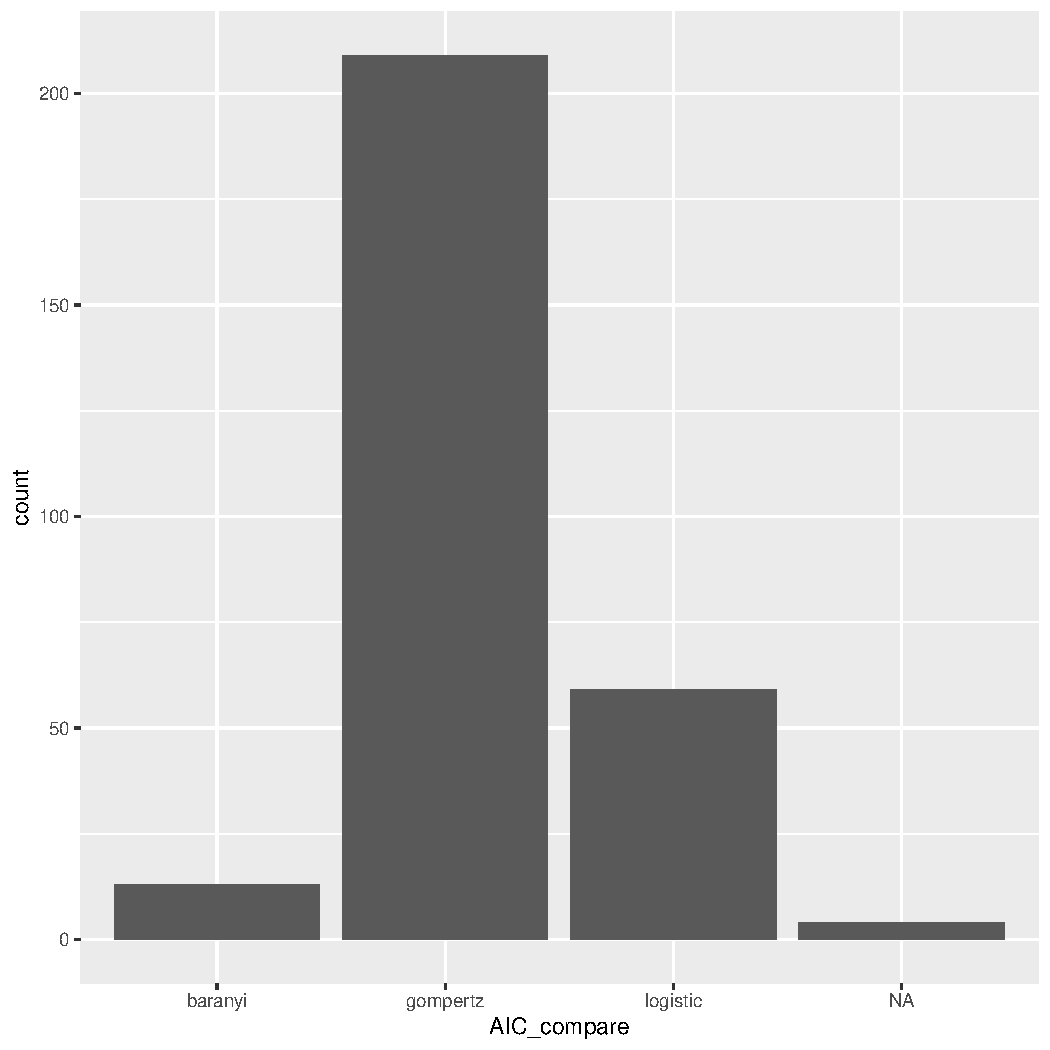
\includegraphics[scale = 0.5]{AIC_plot.pdf}
			\end{minipage}%
			\begin{minipage}{.5\textwidth}
				\centering
				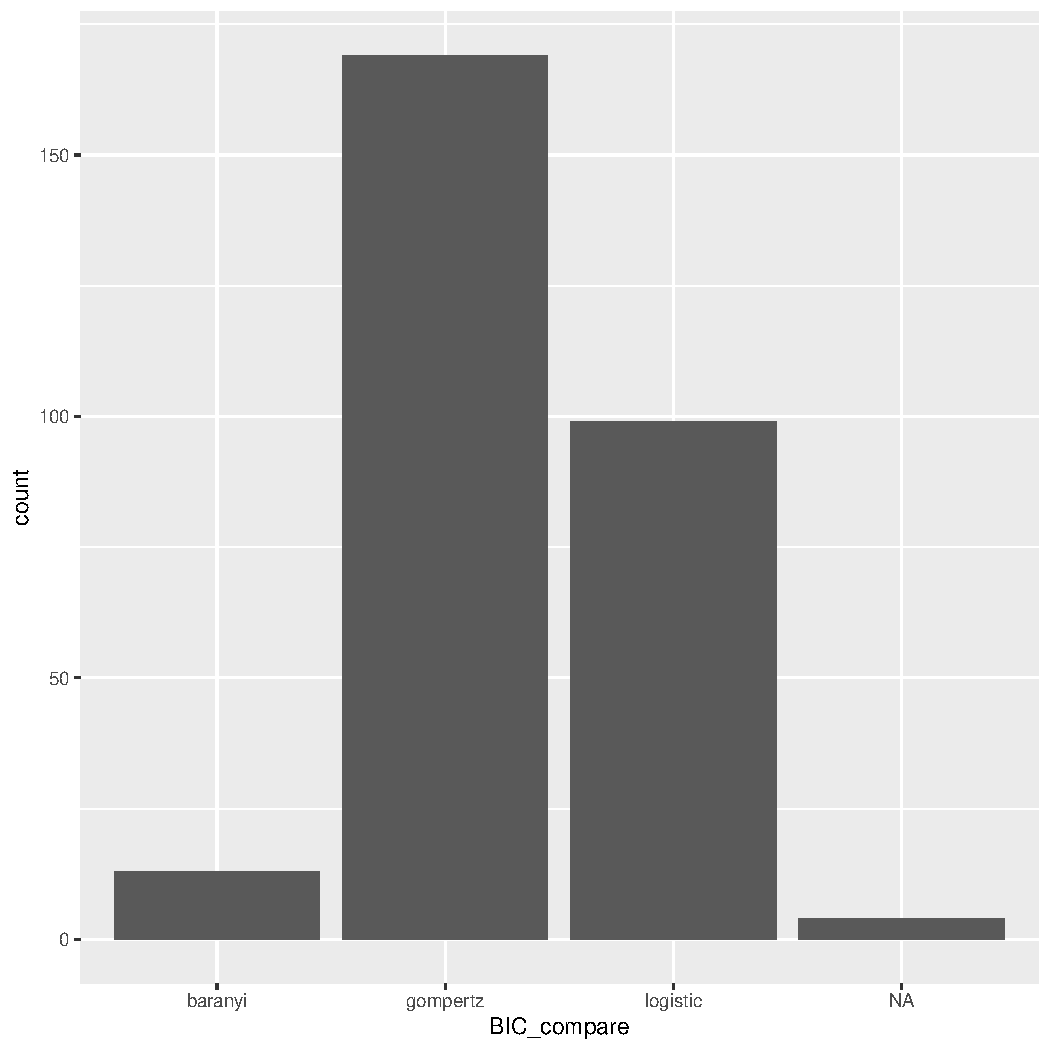
\includegraphics[scale = 0.5]{BIC_plot.pdf}
			\end{minipage}
			\end{center}
		\caption{AIC and BIC comparison}
		\end{figure}
		
		\noindent Now we proceed to the numerical comparison using AIC and BIC calculation. It can be seen that both criterions have shown similar results, with the Gompertz model have the highest frequency of having the minimum value among all the chosen models. It is also worth mentioning that the linear models are also included, but since the results are usually not the best fit, there is no frequency of linear models having the lowest value. Therefore, we can conclude that the non-linear models fits data better than linear models in general, with the Gompertz model fitting the best.

	\pagebreak
	\section{Discussion}
	
	\subsection{Findings and implications}
	
	As shown in the results above, the performance of Quadratic and Cubic linear models are usually not able to predict the full trend in general. Although these models can predict the death phase, the overall AIC and BIC of linear models are higher than others. This could be because bacterial growth could usually be affected by various factors which may not be captured in the mathematical functions \cite{Sutherland and Norris}. For example, though both linear models show a good pattern for the exponential growth phase by the mathematical definition of expressions, both fail to catch the lag phase before the start of cell division. This is because though there has been evidence showing the possibility of cells needing time to divide, the models based on theory usually do not take the lag time into consideration, which causes the inaccuracy when studying the lag phase. By contrast, since it has been observed from laboratory data that the lag phase does exist before the start of exponential growth \cite{Rolfe et al.}Rolfe et al., 2019), the models based on phenomenological data usually provide better performance on the prediction of lag phase. Our result from the non-linear models can prove this. Though the fitting of the Baranyi model for the lag phase shows a slight deviation from the actual point, it could be due to several reasons:
	\begin{itemize}
	\item The current studies on the lag phase are still not sufficient enough that the models cannot fit all lag phases well \cite{Rolfe et al.}. Due to the lack of data for the underlying molecular behavior and physiological processes, current studies on the lag phase is still poor. This could be a potential reason leading to the shortage of theoretical based models when predicting the behaviour of duration before the start of exponential growth.
	\item Another possible reason is the limited sample data for the lag phase. According to Schmidt, the actual lag time has to be determined from the laboratory data instead of model \cite{Yilmaz}. Nevertheless, it is noticed that there are only a few points at the lag phase in our dataset, which could be a possible reason for an inaccurate estimate of the model.
	\end{itemize}
	\noindent For the estimate of the stationary phase, the performance of models is close. In general, most models provide a reasonable pattern for the stationary duration, while the Baranyi model displays some deviation from the data. There are fluctuations shown in the Baranyi model even when the abundance becomes stationary. In this situation, the linear models have a better performance, while the Gompertz and Logistic models are also able to provide an accurate estimation. At the stationary stage, it is hard to distinguish which model has the best estimate.
	\bigbreak
	\noindent It is worth mentioning that one advantage of the models based on population growth theory is that these models seem able to predict the death phase better than the Gompertz and Logistic models. For this estimation, although the Baranyi model also takes death phase into consideration, the overall estimate does not have a close fit. The Gompertz and Logistic model reaches the maximum and stays almost constant without extending beyond the stationary phase \cite{whiting}. This may be due to the empirical nature of these model equations where the death phase is not taken into account \cite{Choudhury}. By comparison, both quadratic and cubic equations are able to provide an accurate estimate for the decline of abundance after stationarity according to our results. The original nature of the mathematical equations could be a reason for this, which could contain both increase and decline in a duration. We can therefore conclude that the equations based on pure mathematical theories can sometimes also be useful, but the situation would be specific and may not be suitable for every case. Though the models derived by phenomenal data are generally more suitable, the situation varies with the different parameter taken into account when deriving the final modelling equation. 
	\bigbreak
	\noindent In addition, it is also noticeable that the sample size and the standard deviation are also factors that could influence the performance of models. We observe that the Baranyi model was not included in the graph for larger sample size and standard deviation in both Figure 3 and Figure 5. This is due to the lack of data, which is caused by the poor fit of the model in this subset. It can be concluded that the range of dataset that the Baranyi model can fit is comparatively smaller than the other models. All the other chosen models have a reasonable fit to the data with different standard deviation, while the linear models show an inaccuracy for the estimation of larger dataset with greater sample size. 
	\bigbreak
	\noindent In general, we can conclude that the overall performance of the modified Gompertz model has the best estimation for our dataset. Models based on the phenomenological data usually are able to provide a better estimate as these are collected from the reality and could provide better estimate, with the parameters counted being an important factor of the effectiveness and comprehensiveness of the model. 
	
	\subsection{Shortcomings}
	
	Though several models have been conducted for our study, it is not comprehensive enough and further work still needs to be done to cover the gap. There are several shortcomings of this study:
	\begin{itemize}
	\item Changes in the environment not taken into account
	\bigbreak
	\noindent Though it is possible to predict the population growth rate, the environment is still likely to alter, which could bring unexpected change in population \cite{Sutherland and Norris}. For example, there are several factors that could potentially influence the bacterial growth, including the temperature, pH value, etc. \cite{Gale} However, uncertainties could be caused by the change of environment during the data collection process while might not be included in the data. This would be a potential cause for the deviation of the modelling, and could lead to different results in the model performances.
	\item Possible inaccuracy by data process
	\bigbreak 
	\noindent In this study, the raw data of the cell population and time are both transformed to their absolute value for further calculation to ensure that the data is relistic. However, there is a possibility to misunderstand the data with negative value at their initial state.
	\bigbreak
	\item Difference in definition of parameters
	\noindent According to the study of \cite{Perni}, the definition of the parameters are usually determinant to the suitability of the models. In our study, the models are all compared with the same starting point to ensure that they are all with the same standard. However, there are some parameters that could slightly differ from other models, which is not taken into consideration in our study. This could also be a potential cause for inaccuracy and further studies need to be conducted to study about this.
	\end{itemize}
	
	\section{Conclusion}
	
	In this study, we have applied the Baranyi model, the modified Gompertz model and the Logistic model with comparison to the Quadratic and the Cubic linear model to find the model of the best estimate for the functional response data across different species. The results have suggested that the modified Gompertz model has the best performance in general, despite the fact that the death phase estimation is not considered. Despite the observation that the mechanical models could be effective when providing prediction after the exponential growth, the models based on phenomenological theories are more suitable for the overall estimates due to the possible reason that these models are derived from realistic data and more features in reality could be taken into consideration. 
	\pagebreak
	\section{Reference list}

\bibliographystyle{apalike}
\end{document}  